\chapter{How I Turned Negative \$20 Million Into \$3.3 Billion}

We begin as the interview begins: not from first principles, but from a finished result that demands explanation. A brief street encounter has already established the speaker as a billionaire who built and sold a hospitality company; the return visit to Beverly Hills is therefore not discovery but reopening. What follows is a spoken master class in business arithmetic: distressed initial condition, scale, trust, cashflow under shock, and the strange way a founder's attention can become an operating advantage. There are no surviving board equations to reproduce, so the mathematics here is deliberately modest and transcript-led.

\section{Cold Open, Turnaround, and the Promise of a Master Class}

The host's opening move is to restage the earlier viral encounter. He reminds us that the first exchange happened on the street, that it spread to an enormous audience, and that it left one question unanswered: how does a person go from a broken position in business to a multibillion-dollar outcome? Before any doctrine is stated, both host and speaker stress that the exchange is unscripted and real. That matters, because the lecture wants the eventual principles to emerge from the same unvarnished register as the stories.

The chapter's first arithmetic is given almost at once:
\begin{align}
E_0 &\approx -\$20\,\mathrm{M},\\
EV_{\mathrm{exit}} &\approx \$3.3\,\mathrm{B},\\
N_{\mathrm{countries}} &= 35.
\end{align}
We shall use \(E_0\) for the distressed starting economic position in the hospitality business, and \(EV_{\mathrm{exit}}\) for the Hilton transaction value cited in the interview. The transcript momentarily passes through a confused phrase---``\$2.2 billion, \$3.3 billion equity value''---and then immediately corrects to enterprise value. The correction matters, so we follow it.

\begin{definition}
The standard accounting identity behind the corrected phrase is
\begin{equation}
EV=\text{Equity Value}+\text{Debt}-\text{Cash}.
\end{equation}
This equation is not derived in the interview; it is the canonical form that explains why enterprise value is the cleaner object here.
\end{definition}

So the interview opens with a state change rather than with a résumé. The host's promise of ``a billion dollars worth of game'' is clumsy in phrase but precise in function: it turns spectacle into a demand for mechanism.

\begin{figure}[h]
\centering
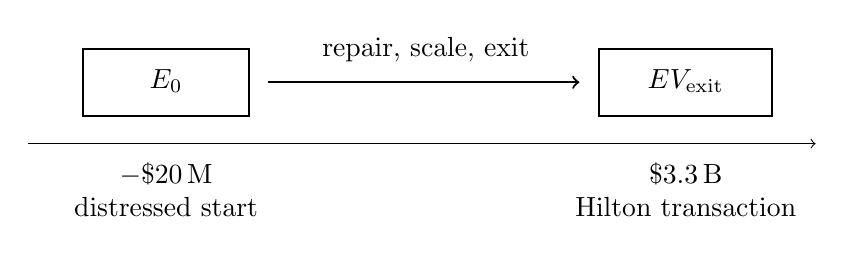
\begin{tikzpicture}[x=1cm,y=1cm]
\draw[->] (0,0) -- (10,0);
\draw[thick] (0.7,0.35) rectangle (2.8,1.2);
\node at (1.75,0.8) {$E_0$};
\node[align=center] at (1.75,-0.58) {$-\$20\,\mathrm{M}$\\distressed start};
\draw[->,thick] (3.05,0.78) -- (7.0,0.78);
\node at (5.05,1.2) {repair, scale, exit};
\draw[thick] (7.25,0.35) rectangle (9.45,1.2);
\node at (8.35,0.8) {$EV_{\mathrm{exit}}$};
\node[align=center] at (8.35,-0.58) {$\$3.3\,\mathrm{B}$\\Hilton transaction};
\end{tikzpicture}
\caption{A transcript-backed value ladder. The figure is an editorial reconstruction of the opening contrast, not a cap-table calculation.}
\end{figure}

\section{Fixing Broken Systems: From Hospitality Turnaround to Brand USA}

The host's first serious follow-up is not about the sale itself, but about what the speaker thinks he has been doing with his life. The answer is immediate and emphatic: fixing broken systems. This is the proper next step in the lecture. If we remained at the level of the exit, we would learn only a terminal price. The speaker wants to move us toward the operating path.

That is why he pivots so quickly from Hilton to Brand USA, to tourism, to service, and to the Oval Office. The point is not self-congratulation. On the contrary, he insists on the opposite: no trophies, no red carpet, no pride of authorship, only the satisfaction of making others look good and of producing results. In this register, value is built by causing institutions to work better for their customers.

When he says that the return on investment in Brand USA was ``outsized,'' the natural bookkeeping object is
\begin{equation}
\mathrm{ROI}=\frac{\text{incremental gain}-\text{cost}}{\text{cost}}.
\end{equation}
The interview does not provide numerical inputs for this ratio, so the expression serves only as clarification. But that clarification matters. The claim is not that the project was prestigious. The claim is that it paid.

The section also widens the speaker's self-description. He once thought he would become a surgeon; he passed instead through shopping centers, hotels, politics, and policy. One line in the transcript is garbled, but its meaning is clear enough: service must be legible from the bottom of the institution to the top of it. That ethic returns later in the hotel business in a very concrete form.

A short sequence near the end of this opening stretch is easy to lose if one writes too abstractly. The speaker recalls \emph{Undercover Boss}, says it did not hurt his brand, and explains why: it made him listen better to his team and to his customers. Then comes a sentence that is as close to an axiom as this lecture gets: it is not what we think or what management thinks that decides the matter; it is what the customer thinks. Only after establishing that principle does he mention his run for governor of California. The host then says, in effect: good, let us make this into a master class. Only then do we turn backward to the first hotel.

\section{Building the First Hotel Without Knowing How}

The lecture now narrows from general identity to technical apprenticeship. The host first misnames the project and is corrected: not Twin Towers, but Polo Towers. The correction matters because the lecture is about to descend into the actual texture of a first large build, and here names, costs, and mistakes all matter.

The speaker says he had never built a hotel. He had built shopping centers, and one of those shopping-center projects had gone wrong in nearly every imaginable way. Contractors went broke. Lumber was paid for twice. Lien releases were not understood. Tenants failed. The economy was collapsing. A retaining wall, absent from the original plans, suddenly had to be built at great cost. The lecture does not sentimentalize this ignorance. It prices it.

That is why the next distinction is so important. He lost the shopping center, but he did not go broke. In the logic of the chapter, that is the first real theorem of survival: we may lose an asset and still preserve the right to learn. It is this preservation of agency that allows the later hotel to be built at all.

The speaker then states the next milestone in the plainest available way:
\begin{equation}
a_{\mathrm{Polo}}\approx 29.
\end{equation}
At roughly that age, he says, he designed and built Polo Towers in Las Vegas. He further describes it as the largest hotel-timeshare complex ever built at one time in the world. We keep that as a speaker's superlative claim. The analytically important sequence is simpler and stronger: ignorance, forced learning, survival, execution.

\subsection{Question \& Answer}

\paragraph{Question.}
How do we build something we do not yet know how to build?

\paragraph{Answer.}
The lecture's answer is severe and practical.
\begin{enumerate}
\item First, we admit that ignorance is real and costly.
\item Next, we go to the object itself: plans, releases, site conditions, missing costs.
\item Then we survive long enough for error to become instruction rather than extinction.
\item Only after that do we earn the right to speak about courage.
\end{enumerate}
The interview rejects the fantasy that nerve can replace diligence. Nerve is required, but mainly to remain present while diligence is painfully assembled.

The passage closes in a way that the lecture does not overdramatize: the project was done with his father, on time and on budget, and it succeeded. The host then asks the right follow-up. Starting at twenty-nine, what relationships or principles made such a project possible? The answer begins unexpectedly not with financiers or contractors, but with the customer.

\section{Brand as Design Choice and Legal Asset}

Once the construction question has been posed, the lecture shifts from the mechanics of building to the problem of fit. The speaker says he always kept things fresh and always listened to the customer. Then he gives a specific example. The project carried the word ``Polo,'' which suggests refinement and exclusivity, but the intended customer base was broad. The challenge, then, was to make the name elevate the project without making the customer feel unwelcome.

This is the first full appearance of brand in the chapter's chronology. Brand is not yet a stock of trust. It is first a design constraint. One chooses a name. One infers what world that name evokes. One then alters the built environment so that the customer is not pushed away by the implication. The speaker says explicitly that the look was not to be the old, staid English version one might expect. It was to be modern.

The Ralph Lauren dispute sharpens the point. The lecture presents the name as something legally defensible, costly to defend, and therefore economically real. The mark had been secured for hotel, timeshare, and casino use. Litigation followed. Serious money was spent. The name was retained. The sequence here is exact and worth preserving:
\begin{enumerate}
\item customer fit,
\item aesthetic execution,
\item legal protection,
\item long-horizon brand value.
\end{enumerate}
Trademarks and domains appear in the lecture not as vanity objects, but as instruments for stabilizing the commercial identity of the project.

At this point the host steps out for a brief mentorship appeal. It should not dominate the notes, but it should not vanish either, because it marks a genuine pause in the rhythm. The interview then resumes in a different room, and the register changes. Up to now we have mainly been discussing the outer formation of a business. The next movement will ask how the operator is formed from within.

\section{Adversity, Presence, and Leadership Discipline}

The new room contains a visible prompt: Iron Man. The host points to it, and the speaker answers with a story of being hit by a car, surviving, healing, and acquiring the nicknames Iron Man and Wolverine. But the lecture does not linger on toughness as spectacle. The story is immediately transformed into a principle: stay present. The speaker contrasts life in the past, life in the future, and life in the present, and then gives the operational consequence. Opportunity appears when attention is real.

This is the right place for the lecture to become more explicit about brand, because the argument is that brand is not maintained by image management alone. It is maintained by a way of being in the room. To formalize the point cautiously, let
\begin{definition}
\(B_t\) denote the stock of brand trust at time \(t\). This stock includes remembered integrity, disciplined execution, and the repeated experience of being treated with respect.
\end{definition}
Then the interview's verbal doctrine can be written as an update rule:
\begin{equation}
B_{t+1}=B_t+\Delta B_t.
\end{equation}
The crucial asymmetry is the one the speaker stresses:
\begin{equation}
\Delta B_t^{+}\ \text{is slow and cumulative},\qquad
\Delta B_t^{-}\ \text{can be large and immediate}.
\end{equation}
This is the mathematical form of the claim that a brand takes decades to build and minutes to kill.

\begin{figure}[h]
\centering
\begin{tikzpicture}[x=1cm,y=1cm]
\draw[->] (0,0) -- (10,0);
\draw[->] (0,0) -- (0,4.2);
\node at (9.55,-0.35) {time};
\node[rotate=90] at (-0.45,3.35) {brand trust};
\draw[thick] (0.6,0.45) -- (1.8,0.82) -- (3.6,1.45) -- (5.4,2.1) -- (7.4,3.0);
\draw[thick] (7.4,3.0) -- (8.2,0.85);
\node at (4.0,2.65) {slow build};
\node at (8.55,2.2) {trust break};
\end{tikzpicture}
\caption{A transcript-backed reconstruction of the lecture's brand asymmetry. What accumulates slowly may be damaged rapidly.}
\end{figure}

\subsection{Question \& Answer}

\paragraph{Question.}
If brand takes decades to build and minutes to kill, what exactly is being accumulated?

\paragraph{Answer.}
Not mere recognition. What accumulates is credibility under repetition. The lecture names the ingredients again and again: integrity, discipline, respect, customer surplus, and the refusal to lie. A brand is therefore not just what is said about the firm. It is the memory of how the firm behaves when choice is available.

The lecture then moves to one of its hardest claims. The speaker says he had to fire the number one salesperson in the world because that person created a cancer in the organization. Everyone told him not to do it. He did it anyway. The reported result was
\begin{equation}
g_{\mathrm{post\text{-}removal}}\approx 20\%.
\end{equation}
We treat that as a speaker-attributed performance claim, not as a clean causal estimate. Yet it belongs in the notes because it reveals the lecture's hierarchy of variables. Short-run revenue is not the only variable in the system. Culture and trust are state variables too.

\subsection{Question \& Answer}

\paragraph{Question.}
Why can removing a top performer make the company grow?

\paragraph{Answer.}
Because a top performer may be locally productive and globally corrosive. If that person teaches the organization to violate its own brand, then the apparent gain is being financed by internal decay. In the lecture's language, leadership means holding the line even when the short-run numbers tempt us not to. The removal hurts a part and saves a system.

\section{Speedboat Versus Battleship: Founder Control Across the Operating Chain}

After a comic detour involving literal brass balls, the host returns to an earlier question and asks again how the first hotel was built. This time the answer comes from a higher altitude. The speaker does not describe site pain or retaining walls. He describes due diligence. He went around to great hotels, studied Four Seasons, Ritz-Carlton, and Marriott, and compared what worked with what did not.

That second answer is important because it complements the first. Section 3 gave us the painful apprenticeship of not knowing how to build. This section gives us the deliberate comparative study that turns pain into method. The speaker says there was a lane for an entrepreneur because the large incumbents had become too corporate. They had rules, scale, and power, but not the founder's direct contact with the guest or with the script of the front desk.

The lecture condenses this distinction into a memorable image. A founder-led company, if properly built, can become a battleship that moves like a speedboat. The compact mathematical version is
\begin{equation}
R_{\mathrm{founder\text{-}led}} > R_{\mathrm{bureaucratic}},
\end{equation}
where \(R\) denotes responsiveness. This is not a measured inequality. It is a disciplined shorthand for the speaker's comparison between entrepreneurial flexibility and bureaucratic drag.

\begin{figure}[h]
\centering
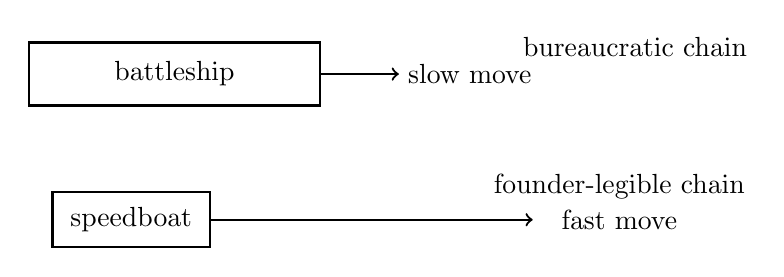
\begin{tikzpicture}[x=1cm,y=1cm]
\draw[thick] (0.5,2.45) rectangle (4.2,3.25);
\node at (2.35,2.85) {battleship};
\draw[->,thick] (4.2,2.85) -- (5.2,2.85);
\node at (6.1,2.85) {slow move};

\draw[thick] (0.8,0.65) rectangle (2.8,1.35);
\node at (1.8,1.0) {speedboat};
\draw[->,thick] (2.8,1.0) -- (6.9,1.0);
\node at (8.0,1.0) {fast move};

\node at (8.2,3.2) {bureaucratic chain};
\node at (8.0,1.42) {founder-legible chain};
\end{tikzpicture}
\caption{The lecture's contrast between scale without agility and scale with founder-legible control. The image is verbal in the interview and diagrammatic here.}
\end{figure}

The section becomes especially concrete at this point, and that concreteness should not be cleaned away. The speaker says he could write code for back-of-house systems, speak tax and facilities management, make a bed, specify towel placement, and place a tent card under beds saying they had been cleaned there too. This is not decorative humility. It is a claim about what gives authority to delegation. Delegation is not rejected in the lecture; blind delegation is.

\paragraph{A second operating principle.}
The founder may coach and scale, but only after making visible that no job in the system lies outside the realm of understanding. This is why the speaker insists that there are, in a deeper sense, no titles. There is only shared service and shared liability to the brand.

\section{Cashflow Shock, Bank Trust, Negotiation Silence, and the State as a Broken Business}

The lecture's last large turn begins with 9/11. Flights are grounded, guests disappear, and the hospitality business is hit not first as an issue of mood but as an issue of inflow. The cash register, as the garbled transcript puts it, effectively goes to zero. This is where the chapter's arithmetic becomes strictest. If operating inflow disappears while obligations remain, then survival depends on liquidity and on the willingness of capital providers to keep believing the story.

A useful reconstruction is
\begin{align}
C_{t+1} &= C_t + F_t + L_t - O_t,\\
F_t &\approx 0 \qquad \text{during the shutdown interval.}
\end{align}
Here \(C_t\) is cash, \(F_t\) operating inflow, \(L_t\) new liquidity raised from lenders, and \(O_t\) continuing obligation. The interview does not present a balance sheet, so the formula is only a bookkeeping frame. But it is the right frame. When \(F_t\) collapses, rhetoric cannot repair the system. Truthful communication and bridge financing can.

\begin{figure}[h]
\centering
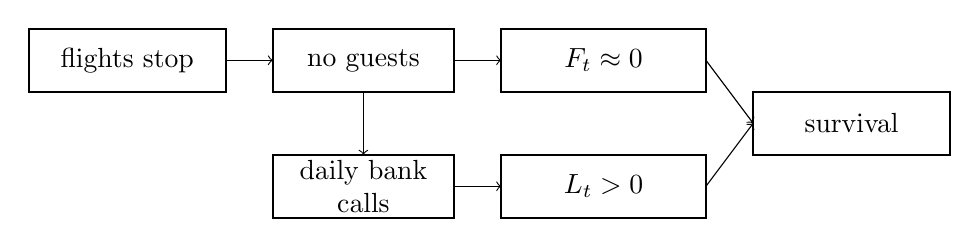
\begin{tikzpicture}[x=1cm,y=1cm]
\draw[thick] (0.0,0.2) rectangle (2.5,1.0);
\node at (1.25,0.6) {flights stop};

\draw[thick] (3.1,0.2) rectangle (5.4,1.0);
\node at (4.25,0.6) {no guests};

\draw[thick] (6.0,0.2) rectangle (8.6,1.0);
\node at (7.3,0.6) {$F_t\approx 0$};

\draw[thick] (3.1,-1.4) rectangle (5.4,-0.6);
\node[align=center] at (4.25,-1.0) {daily bank\\calls};

\draw[thick] (6.0,-1.4) rectangle (8.6,-0.6);
\node at (7.3,-1.0) {$L_t>0$};

\draw[thick] (9.2,-0.6) rectangle (11.7,0.2);
\node at (10.45,-0.2) {survival};

\draw[->] (2.5,0.6) -- (3.1,0.6);
\draw[->] (5.4,0.6) -- (6.0,0.6);
\draw[->] (4.25,0.2) -- (4.25,-0.6);
\draw[->] (8.6,0.6) -- (9.2,-0.2);
\draw[->] (5.4,-1.0) -- (6.0,-1.0);
\draw[->] (8.6,-1.0) -- (9.2,-0.2);
\end{tikzpicture}
\caption{The crisis logic of the 9/11 section. Each box is an editorial reconstruction of a step stated in the interview.}
\end{figure}

\paragraph{A worked liquidity update.}
Suppose, as a pure bookkeeping example, that
\[
C_t=\$10\,\mathrm{M},\qquad O_t=\$6\,\mathrm{M},\qquad F_t=0,\qquad L_t=\$4\,\mathrm{M}.
\]
Then
\begin{align}
C_{t+1} &= C_t + F_t + L_t - O_t\\
&= \$10\,\mathrm{M}+0+\$4\,\mathrm{M}-\$6\,\mathrm{M}\\
&= \$8\,\mathrm{M}.
\end{align}
The point of the example is not the specific number. It is the structure. Crisis survival is a cashflow problem before it is a storytelling problem.

\subsection{Question \& Answer}

\paragraph{Question.}
Why tell the bank the good, the bad, and the ugly instead of negotiating aggressively?

\paragraph{Answer.}
Because in the lecture's framework, future capital depends first on trust. A bank can work with trouble if trouble is described truthfully. It cannot reliably work with concealment. Once trust is broken, forecasting fails, and the relationship becomes unstable. Candor is therefore not softness. It is a capital strategy.

The three C's of banking are presented in exactly that spirit:
\begin{itemize}
\item Capacity,
\item Character,
\item Credit.
\end{itemize}
Character is the hinge term. The lecture's claim is that numbers become finance only when character makes them believable over time.

The negotiation doctrine that follows is a different expression of the same restraint. The speaker says that the first person who talks loses, that one must not talk past the close, and that he once waited a week rather than calling too soon. The sequence may be written schematically as
\begin{equation}
\text{close attempt}\longrightarrow \text{silence}\longrightarrow \text{counterparty response}.
\end{equation}
We should not mistake this for a theorem. It is an attributed operating heuristic whose purpose is to prevent a seller from renegotiating against himself.

Only now does the lecture make its final scale change. The speaker turns to California and treats it as a broken business. The two quantitative anchors given are
\begin{equation}
\operatorname{rank}_{\mathrm{GDP}}(\mathrm{California})=5,\qquad
N_{\mathrm{meetings}}>300.
\end{equation}
The first is a scale marker; the second is an input marker. California is described as country-sized in economic weight, and the speaker says he met with more than three hundred people before concluding that the state was not affordable, livable, or workable.

One should keep the analogy cautious but intact. The lecture is not secretly switching subjects. It is scaling the same grammar upward. The recurring failures are named in terms already familiar from the rest of the chapter:
\begin{itemize}
\item no conversation with the customer,
\item no felt knowledge of payroll,
\item failed execution,
\item overregulation where regulation should have been discriminating rather than suffocating,
\item too little truth from leadership.
\end{itemize}
So the chapter ends exactly where its inner logic points. A person who believes he has spent his life fixing broken businesses now sees a state as one more operating system in need of repair.

\section{Summary}

The lecture begins with a spectacle, but it is not content to remain one. The opening contrast
\[
E_0\approx -\$20\,\mathrm{M},\qquad EV_{\mathrm{exit}}\approx \$3.3\,\mathrm{B}
\]
is treated not as a miracle, but as a problem to be unfolded. First the speaker defines himself as a fixer of broken systems; then he returns to the brutal apprenticeship of not yet knowing how to build; then he shows how customer fit and legal protection enter brand; then he recasts adversity as attention, attention as trust, and trust as a state variable; then he shows how founder knowledge makes a large machine nimble; and finally he moves through crisis liquidity, bank relations, negotiation silence, and the state-as-business analogy.

What makes the chapter mathematically alive is that each business claim is quietly translated into structure. Enterprise value distinguishes itself from equity value. Brand becomes an update rule. Crisis becomes a cash recurrence. Founder control becomes a statement about responsiveness. The lecture therefore unfolds step by step in the proper way: not as a bundle of motivational fragments, but as a sequence of operational updates through which a damaged position is repaired, scaled, protected, financed, and finally generalized into a broader philosophy of leadership.